\documentclass{article}
\usepackage{graphicx}

\begin{document}
	\title{Logic Gates}
	\author{Clement Obieke}

	
	
\maketitle
\newpage
\centering
\section*{Table Of Contents}
	
	\begin{enumerate}
		\item Introduction
		\item Types of Logic Gates and their Truth Tables
		\begin{itemize}
			\item AND Gate
			\item OR Gate
			\item NOT Gate
			\item NOR Gate
			\item NAND Gate
			\item XOR Gate
			\item XNOR Gate
		\end{itemize}
			\item Summary		
	\end{enumerate}
	
	
\newpage
\section{Introduction}
	\raggedright
	\paragraph{}
	Logic gates were fabricated from an array of configurable switches, each consisting of a monolayer of redox-active rotaxanes sandwiched between metal electrodes~\cite{collier1999electronically}.  
	
	A gate in a simple electronic componet that functions like a lightbulb.
	They function by combining multiple signals to produce a single signal 
	based on their unique properties~\cite{okoacha2021logicgatesintro}.
	
\section{Types of Logic Gates}
		\paragraph{1}
		Fundamental gates are AND, OR , NOT:
		\begin{minipage}{\linewidth}
			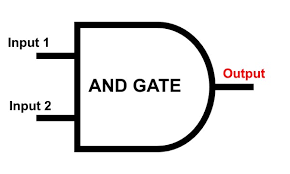
\includegraphics[width = 0.3\linewidth]{and}
			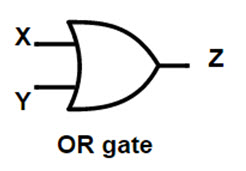
\includegraphics[width = 0.3\linewidth]{or}
			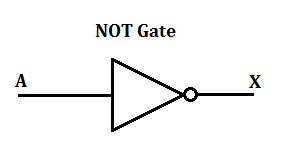
\includegraphics[width = 0.37\linewidth]{not}
		\end{minipage}
		\paragraph{2}
		Derived Gates NAND, NOR, XOR and XNOR(derived from fundamental gates)
		\begin{minipage}{\linewidth}
			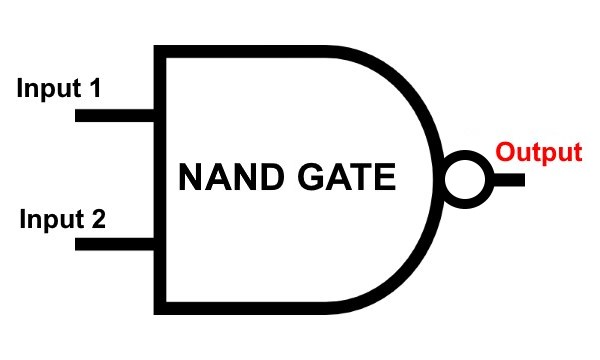
\includegraphics[width = 0.2\linewidth]{nand}
			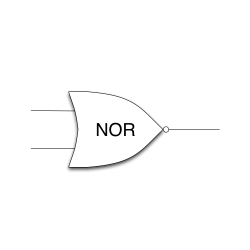
\includegraphics[width = 0.3\linewidth, height=0.15\textheight]{nor}
			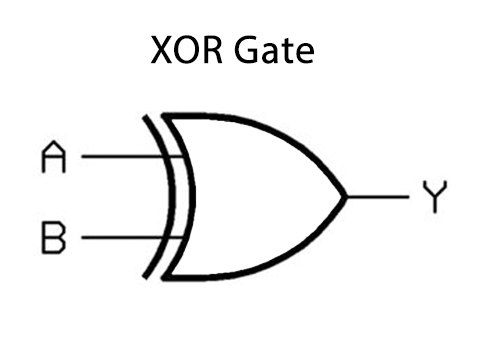
\includegraphics[width = 0.2\linewidth]{xor}
			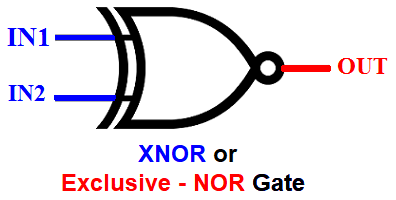
\includegraphics[width = 0.2\linewidth]{xnor}
		\end{minipage}
		\paragraph{3}
		Universal Gates NAND and NOR gates(The fundamental gates can be realized through them).
		\begin{minipage}{\linewidth}
			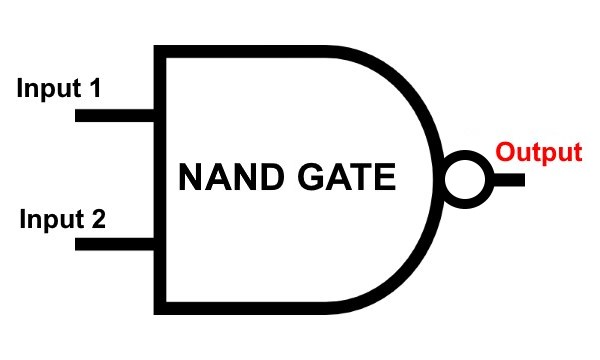
\includegraphics[width = 0.36\linewidth]{nand}
			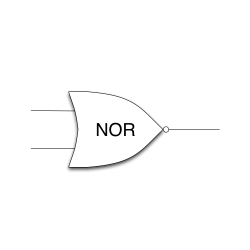
\includegraphics[width = 0.4\linewidth, height=0.23\textheight]{nor}
		\end{minipage}
referenced from~\cite{okoacha2021logicgatestypes}
\subsection{AND Gate}
	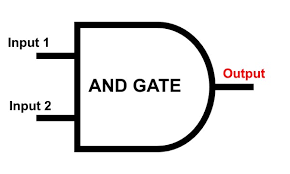
\includegraphics{and}
	\paragraph{}
		The \textbf{AND} operation produces a true output (result of 1) only for a single case when all of the input variables are 1 and a false output(result of 0) where one or more inputs are 0.
		\begin{table}[h]
			\centering
			\label{tab:table1}
			\caption{AND Logic Table}
			\begin{tabular}{|c|c|c|}
				INPUT 1 & INPUT 2 & OUTPUT\\
				\hline
				1&1&1\\
				1&0&0\\
				0&1&0\\
				0&0&0\\
			\end{tabular}
		\end{table}
		
\newpage
\subsection{OR Gate}
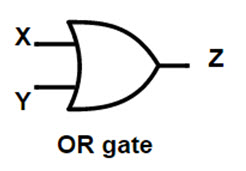
\includegraphics{or}
\paragraph{}
The \textbf{OR} operation produces a true output (result of 1)when any of the input variables are 1 and a false output(result of 0) where both inputs are 0.
\begin{table}[h]
	\centering
	\label{tab:table2}
	\caption{OR Logic Table}
	\begin{tabular}{|c|c|c|}
		INPUT 1 & INPUT 2 & OUTPUT\\
		\hline
		1&1&1\\
		1&0&1\\
		0&1&1\\
		0&0&0\\
	\end{tabular}
\end{table}

\newpage
\subsection{NOT Gate}
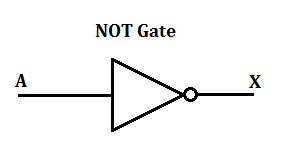
\includegraphics{not}
\paragraph{}
The \textbf{NOT} operation also known as a \textbf{logical inverter}, has only one input and produces the oppostite of the input signal.
\begin{table}[h]
	\centering
	\label{tab:table3}
	\caption{NOT Logic Table}
	\begin{tabular}{|c|c|}
		INPUT & OUTPUT\\
		\hline
		1&0\\
		0&1\\
	\end{tabular}
\end{table}

\newpage 
\subsection{NOR Gate}
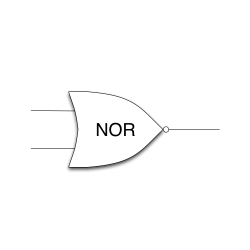
\includegraphics{nor}
\paragraph{}
The \textbf{NOR} operation produces the opposite result of an OR Gate.
\begin{table}[h]
	\centering
	\label{tab:table4}
	\caption{NOR Logic Table}
	\begin{tabular}{|c|c|c|}
		INPUT 1 & INPUT 2 & OUTPUT\\
		\hline
		1&1&0\\
		1&0&0\\
		0&1&0\\
		0&0&1\\
	\end{tabular}
\end{table}

\newpage

\subsection{NAND Gate}
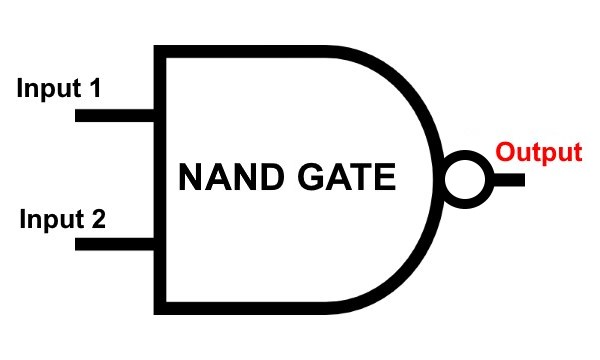
\includegraphics[width=0.7\linewidth]{nand}
\paragraph{}
The \textbf{NAND} operation produces the opposite output of an AND Gate.
\begin{table}[h]
	\centering
	\label{tab:table5}
	\caption{NAND Logic Table}
	\begin{tabular}{|c|c|c|}
		INPUT 1 & INPUT 2 & OUTPUT\\
		\hline
		1&1&0\\
		1&0&1\\
		0&1&1\\
		0&0&1\\
	\end{tabular}
\end{table}

\newpage
\subsection{XOR Gate}
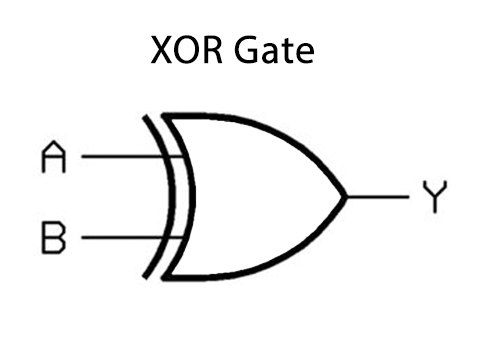
\includegraphics[width=0.8\linewidth]{xor}
\paragraph{}
The \textbf{XOR} operation produces a true output (result of 1) if either case of the input variables are 1 and a false output(result of 0) if both inputs are 0 or one at the same time.
\begin{table}[h]
	\centering
	\label{tab:table6}
	\caption{AND Logic Table}
	\begin{tabular}{|c|c|c|}
		INPUT 1 & INPUT 2 & OUTPUT\\
		\hline
		1&1&0\\
		1&0&1\\
		0&1&1\\
		0&0&0\\
	\end{tabular}
\end{table}

\newpage
\subsection{XNOR Gate}
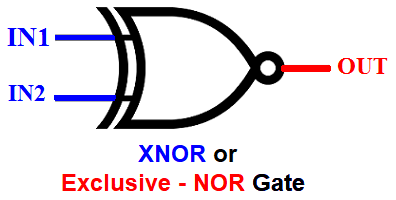
\includegraphics[width=0.8\linewidth]{xnor}
\paragraph{}
The \textbf{XNOR} operation produces the opposite output of the operation XOR Gate
\begin{table}[h]
	\centering
	\label{tab:table7}
	\caption{XOR Logic Table}
	\begin{tabular}{|c|c|c|}
		INPUT 1 & INPUT 2 & OUTPUT\\
		\hline
		1&1&1\\
		1&0&0\\
		0&1&0\\
		0&0&1\\
	\end{tabular}
\end{table}
Referenced from~\cite{okoacha2021logicgatestype2}
\newpage
\section{Summary}

In a nutshell, Logic Gates are basic computer components used in the design of logical componets. They are used in various complex combinations and connections to perform operations. They are implemented in various technologies and from the foundation for computers.

\newpage

\bibliography{gst108}
\bibliographystyle{ieeetr}

\end{document}